\newpage
\appendix

\section{Non-Markovian Forward Processes for a Discrete Case}
\label{app:discrete}
In this section, we describe a non-Markovian forward processes for discrete data and corresponding variational objectives. Since the focus of this paper is to accelerate reverse models corresponding to the Gaussian diffusion, we leave empirical evaluations as future work. 

For a categorical observation $\vx_0$ that is a one-hot vector with $K$ possible values, we define the forward process as follows. First, we have $q(\vx_t | \vx_0)$ as the following categorical distribution:
\begin{align}
    q(\vx_t | \vx_0) = \mathrm{Cat}(\alpha_t \vx_0 + (1 - \alpha_t) \vone_K)
\end{align}
where $\vone_K \in \R^{K}$ is a vector with all entries being $1/K$, and $\alpha_t$ decreasing from $\alpha_0 = 1$ for $t = 0$ to $\alpha_T = 0$ for $t = T$.
Then we define $q(\vx_{t-1} | \vx_t, \vx_0)$ as the following mixture distribution:
\begin{align}
    q(\vx_{t-1} | \vx_t, \vx_0) = \begin{cases}
    \mathrm{Cat}(\vx_t) & \text{with probability } \sigma_t \\
    \mathrm{Cat}(\vx_0) & \text{with probability } (\alpha_{t-1} - \sigma_t \alpha_t) \\
    \mathrm{Cat}(\vone_K) & \text{with probability } (1 - \alpha_{t-1}) - (1 - \alpha_t) \sigma_t
    \end{cases},
\end{align}
or equivalently:
\begin{align}
    q(\vx_{t-1} | \vx_t, \vx_0) = \mathrm{Cat}\left(\sigma_t \vx_t + (\alpha_{t-1} - \sigma_t \alpha_t) \vx_0 + ((1 - \alpha_{t-1}) - (1 - \alpha_t) \sigma_t) \vone_K\right),
\end{align}
which is consistent with how we have defined $q(\vx_t | \vx_0)$. 

Similarly, we can define our reverse process $p_\theta(\vx_{t-1} | \vx_t)$ as:
\begin{align}
    p_\theta(\vx_{t-1} | \vx_t) = \mathrm{Cat}\left(\sigma_t \vx_t + (\alpha_{t-1} - \sigma_t \alpha_t) f_\theta^{(t)}(\vx_t) + ((1 - \alpha_{t-1}) - (1 - \alpha_t) \sigma_t) \vone_K\right),
\end{align}
where $f_\theta^{(t)}(\vx_t)$ maps $\vx_t$ to a $K$-dimensional vector. As $(1 - \alpha_{t-1}) - (1 - \alpha_t) \sigma_t \to 0$, the sampling process will become less stochastic, in the sense that it will either choose $\vx_t$ or the predicted $\vx_0$ with high probability.
The KL divergence
\begin{align}
    \KL(q(\vx_{t-1} | \vx_t, \vx_0) \Vert p_\theta(\vx_{t-1} | \vx_t))
\end{align}
is well-defined, and is simply the KL divergence between two categoricals. Therefore, the resulting variational objective function should be easy to optimize as well. Moreover, as KL divergence is convex, we have this upper bound (which is tight when the right hand side goes to zero):
\begin{align}
    \KL(q(\vx_{t-1} | \vx_t, \vx_0) \Vert p_\theta(\vx_{t-1} | \vx_t)) \leq (\alpha_{t-1} - \sigma_t \alpha_t) \KL(\mathrm{Cat}(\vx_0) \Vert \mathrm{Cat}(f_\theta^{(t)}(\vx_t))). \nonumber
\end{align}
The right hand side is simply a multi-class classification loss (up to constants), so we can arrive at similar arguments regarding how changes in $\sigma_t$ do not affect the objective (up to re-weighting).

\section{Proofs}
\label{app:proofs}

\begin{lemma}
\label{lemma:reverse-process-consistency}
For $q_\sigma(\vx_{1:T} | \vx_0)$ defined in \eqref{eq:diff-new} and $q_\sigma(\vx_{t-1} | \vx_t, \vx_0)$ defined in \eqref{eq:reversed-close-form}, we have:
\begin{align}
q_\sigma(\vx_{t} | \vx_0) = \gN(\sqrt{\alpha_t} \vx_0, (1 - \alpha_t) \mI)
\end{align}
\end{lemma}
\begin{proof}
Assume for any $t \leq T$, $q_\sigma(\vx_{t} | \vx_0) = \gN(\sqrt{\alpha_t} \vx_0, (1 - \alpha_t) \mI)$ holds, if:
\begin{align}
    q_\sigma(\vx_{t-1} | \vx_0) = \gN(\sqrt{\alpha_{t-1}} \vx_0, (1 - \alpha_{t-1}) \mI)
\end{align}
then we can prove the statement with an induction argument for $t$ from $T$ to $1$, since the base case ($t = T$) already holds.

First, we have that
$$
    q_\sigma(\vx_{t-1} | \vx_0) := \int_{\vx_t} q_\sigma(\vx_{t} | \vx_0) q_\sigma(\vx_{t-1} | \vx_t, \vx_0) \diff \vx_t
$$
and
\begin{gather}
   q_\sigma(\vx_{t} | \vx_0) = \gN(\sqrt{\alpha_t} \vx_0, (1 - \alpha_t) \mI) \\
   q_\sigma(\vx_{t-1} | \vx_t, \vx_0) = \gN\left(\sqrt{\alpha_{t-1}} \vx_{0} + \sqrt{1 - \alpha_{t-1} - \sigma^2_t} \cdot {\frac{\vx_{t}  - \sqrt{\alpha_{t}} \vx_0}{\sqrt{1 - \alpha_{t}}}}, \sigma_t^2 \mI \right).
\end{gather}
From \citet{bishop2006pattern} (2.115), we have that $q_\sigma(\vx_{t-1} | \vx_0)$ is Gaussian, denoted as $\gN(\mu_{t-1}, \Sigma_{t-1})$ where
\begin{align}
    \mu_{t-1} & = \sqrt{\alpha_{t-1}} \vx_{0} + \sqrt{1 - \alpha_{t-1} - \sigma^2_t} \cdot {\frac{\sqrt{\alpha_t} \vx_0  - \sqrt{\alpha_{t}} \vx_0}{\sqrt{1 - \alpha_{t}}}} \\
    & = \sqrt{\alpha_{t-1}} \vx_{0}
\end{align}
and
\begin{align}
    \Sigma_{t-1} & = \sigma_t^2 \mI + \frac{1 - \alpha_{t-1} - \sigma^2_t}{1 - \alpha_t} (1 - \alpha_t) \mI = (1 - \alpha_{t-1}) \mI
\end{align}
Therefore, $q_\sigma(\vx_{t-1} | \vx_0) = \gN(\sqrt{\alpha_{t-1}} \vx_0, (1 - \alpha_{t-1}) \mI)$, which allows us to apply the induction argument.
\end{proof}


\unifiedklobj*

\begin{proof}
From the definition of $J_\sigma$:
\begin{align}
   J_\sigma(\epsilon_\theta) & := \bb{E}_{\vx_{0:T} \sim q(\vx_{0:T})} \left[\log q_\sigma(\vx_T | \vx_0) + \sum_{t=2}^{T} \log q_\sigma(\vx_{t-1} | \vx_t, \vx_0) - \sum_{t=1}^{T} \log p_\theta^{(t)}(\vx_{t-1} | \vx_t) \right] \\
   & \equiv \bb{E}_{\vx_{0:T} \sim q(\vx_{0:T})} \left[\sum_{t=2}^{T} \KL(q_\sigma(\vx_{t-1} | \vx_t, \vx_0)) \Vert p_\theta^{(t)}(\vx_{t-1} | \vx_t)) - \log p_\theta^{(1)}(\vx_0 | \vx_1)  \right] \nonumber
\end{align}
where we use $\equiv$ to denote ``equal up to a value that does not depend on $\epsilon_\theta$ (but may depend on $q_\sigma$)''. For $t > 1$:
\begin{align}
   & \bb{E}_{\vx_{0}, \vx_t \sim q(\vx_{0}, \vx_t)} [\KL(q_\sigma(\vx_{t-1} | \vx_t, \vx_0)) \Vert p_\theta^{(t)}(\vx_{t-1} | \vx_t))] \nonumber \\
   = & \ \bb{E}_{\vx_{0}, \vx_t \sim q(\vx_{0}, \vx_t)}[\KL(q_\sigma(\vx_{t-1} | \vx_t, \vx_0)) \Vert q_\sigma(\vx_{t-1} | \vx_t, f_{\theta}^{(t)}(\vx_t)))] \nonumber \\
   \equiv & \ \bb{E}_{\vx_{0}, \vx_t \sim q(\vx_{0}, \vx_t)}\left[\frac{\norm{\vx_0 - f_{\theta}^{(t)}(\vx_t)}_2^2}{2 \sigma_t^2}\right] \\
   = & \ \bb{E}_{\vx_{0} \sim q(\vx_{0}), \epsilon \sim \gN(\vzero, \mI), \vx_t = \sqrt{\alpha_t} \vx_0 + \sqrt{1 - \alpha_t} \epsilon}\left[\frac{\norm{\frac{{(\vx_t - \sqrt{1 - \alpha_t} \epsilon)}}{\sqrt{\alpha_t}} - \frac{(\vx_t - \sqrt{1 - \alpha_t} \epsilon_{\theta}^{(t)}(\vx_t))}{\sqrt{\alpha_t}}}_2^2}{2 \sigma_t^2}\right] \\
   = & \ \bb{E}_{\vx_{0} \sim q(\vx_{0}), \epsilon \sim \gN(\vzero, \mI), \vx_t = \sqrt{\alpha_t} \vx_0 + \sqrt{1 - \alpha_t} \epsilon}\left[\frac{\norm{\epsilon - \epsilon_{\theta}^{(t)}(\vx_t)}_2^2}{2 d \sigma_t^2 \alpha_t}\right]
\end{align}
where $d$ is the dimension of $\vx_0$. For $t = 1$:
\begin{align}
   & \ \bb{E}_{\vx_{0}, \vx_1 \sim q(\vx_{0}, \vx_1)} \left[ - \log p_\theta^{(1)}(\vx_0 | \vx_1)  \right] \equiv \bb{E}_{\vx_{0}, \vx_1 \sim q(\vx_{0}, \vx_1)}\left[\frac{\norm{\vx_0 - f_{\theta}^{(t)}(\vx_1)}_2^2}{2 \sigma_1^2}\right] \\
   = & \ \bb{E}_{\vx_{0} \sim q(\vx_{0}), \epsilon \sim \gN(\vzero, \mI), \vx_1 = \sqrt{\alpha_1} \vx_0 + \sqrt{1 - \alpha_t} \epsilon}\left[\frac{\norm{\epsilon - \epsilon_{\theta}^{(1)}(\vx_1)}_2^2}{2 d \sigma_1^2 \alpha_1}\right]
\end{align}
Therefore, when $\gamma_t = 1 / (2 d \sigma_t^2 \alpha_t)$ for all $t \in \{1, \ldots, T\}$, we have
\begin{align}
    J_\sigma(\epsilon_\theta) \equiv \sum_{t=1}^{T} \frac{1}{2 d \sigma_t^2 \alpha_t} \bb{E}\left[\norm{\epsilon_{\theta}^{(t)}(\vx_t) - \epsilon_t}_2^2 \right] = L_\gamma(\epsilon_\theta)
\end{align}
for all $\epsilon_\theta$. From the definition of ``$\equiv$'', we have that $J_\sigma = L_\gamma + C$.
\end{proof}

\equivalence*

\begin{proof}
In the context of the proof, we consider $t$ as a continous, independent ``time'' variable and $\vx$ and $\alpha$ as functions of $t$. First, let us consider a reparametrization between DDIM and the VE-SDE\footnote{Refer to \citep{song2020score} for more details of VE-SDE.} by introducing the variables $\bar{\vx}$ and $\sigma$:
\begin{align}
    \bar{\vx}(t) = \bar{\vx}(0) + \sigma(t) \epsilon, \quad \epsilon \sim \gN(0, \mI),
\end{align}
for $t \in [0, \infty)$ and an increasing continuous function $\sigma: \bb{R}_{\geq 0} \to \bb{R}_{\geq 0}$ where $\sigma(0) = 0$. 

We can then define $\alpha(t)$ and $\vx(t)$ corresponding to DDIM case as:
\begin{gather}
    \bar{\vx}(t) = \frac{\vx(t)}{\sqrt{\alpha(t)}} \\
    \sigma(t) = \sqrt{\frac{1 - \alpha(t)}{\alpha(t)}}.
\end{gather}
This also means that:
\begin{gather}
    \vx(t) = \frac{\bar{\vx}(t)}{\sqrt{\sigma^2(t) + 1}} \\
    \alpha(t) = \frac{1}{1 + \sigma^2(t)},
\end{gather}
which establishes an bijection between $(\vx, \alpha)$ and $(\bar{\vx}, \sigma)$. From \Eqref{eq:reparam_xt} we have (note that $\alpha(0) = 1$):
\begin{align}
    \frac{\vx(t)}{\sqrt{\alpha(t)}} = \frac{\vx(0)}{\sqrt{\alpha(0)}} + \sqrt{\frac{1 - \alpha(t)}{\alpha(t)}} \epsilon, \quad \epsilon \sim \gN(0, \mI)
\end{align}
which can be reparametrized into a form that is consistent with VE-SDE:
\begin{align}
    \bar{\vx}(t) = \bar{\vx}(0) + \sigma(t) \epsilon.
\end{align}

Now, we derive the ODE forms for both DDIM and VE-SDE and show that they are equivalent.

\paragraph{ODE form for DDIM} We repeat \Eqref{eq:ddim-euler} here:
\begin{align}
    \frac{\vx_{t-\Delta t}}{\sqrt{\alpha_{t-\Delta t}}}  = \frac{\vx_t}{\sqrt{\alpha_t}}  + \left(\sqrt{\frac{1 - \alpha_{t-\Delta t}}{\alpha_{t-\Delta t}}} - \sqrt{\frac{1 - \alpha_{t}}{\alpha_t}}\right) \epsilon_\theta^{(t)}(\vx_t),
\end{align}
which is equivalent to:
\begin{align}
    \bar{\vx}(t-\Delta t) = \bar{\vx}(t) + (\sigma(t-\Delta t) - \sigma(t)) \cdot \epsilon_\theta^{(t)}(\vx(t))
\end{align}
Divide both sides by $(-\Delta t)$ and as $\Delta t \to 0$, we have:
\begin{align}
    \frac{\diff \bar{\vx}(t)}{\diff t} = \frac{\diff \sigma(t)}{\diff t} \epsilon_\theta^{(t)}\left(\frac{\bar{\vx}(t)}{\sqrt{\sigma^2(t) + 1}}\right), \label{eq:ddim:differential}
\end{align}
which is exactly what we have in \Eqref{eq:ddim-ode}. 

We note that for the optimal model, $\epsilon_\theta^{(t)}$ is a minimizer:
\begin{align}
    \epsilon_\theta^{(t)} = \argmin_{f_t} \bb{E}_{\vx(0) \sim q(\vx), \epsilon \sim \gN(0, \mI)}[\norm{f_t(\vx(t)) - \epsilon}_2^2] \label{eq:dsm-ddim}
\end{align}
where $\vx(t) = \sqrt{\alpha(t)} \vx(t) + \sqrt{1 - \alpha(t)} \epsilon$.

\paragraph{ODE form for VE-SDE} Define $p_t(\bar{\vx})$ as the data distribution perturbed with $\sigma^2(t)$ variance Gaussian noise. The probability flow for VE-SDE is defined as \cite{song2020score}:
\begin{align}
    \diff \bar{\vx} = -\frac{1}{2} g(t)^2 \nabla_{\bar{\vx}} \log p_t(\bar{\vx}) \diff t  \label{eq:yang-ode}
\end{align}
where $g(t) = \sqrt{\frac{\diff \sigma^2(t)}{\diff t}}$ is the diffusion coefficient, and $\nabla_{\bar{\vx}} \log p_t(\bar{\vx})$ is the score of $p_t$. 

The $\sigma(t)$-perturbed score function $\nabla_{\bar{\vx}} \log p_t(\bar{\vx})$ is also a minimizer (from denoising score matching~\citep{vincent2011connection}):
\begin{align}
    \nabla_{\bar{\vx}} \log p_t = \argmin_{g_t} \bb{E}_{\vx(0) \sim q(\vx), \epsilon \sim \gN(0, \mI)}[\norm{g_t(\bar{\vx}) + \epsilon / \sigma(t)}_2^2] \label{eq:dsm-ve}
\end{align}
where $\bar{\vx}(t) = \bar{\vx}(t) + \sigma(t) \epsilon$. 

Since there is an equivalence between $\vx(t)$ and $\bar{\vx}(t)$, we have the following relationship:
\begin{gather}
    \nabla_{\bar{\vx}} \log p_t(\bar{\vx}) = - \frac{\epsilon_\theta^{(t)}\left(\frac{\bar{\vx}(t)}{\sqrt{\sigma^2(t) + 1}}\right)}{\sigma(t)} \label{eq:score-equivalence}
\end{gather}
from \Eqref{eq:dsm-ddim} and \Eqref{eq:dsm-ve}. Plug \Eqref{eq:score-equivalence} and definition of $g(t)$ in \Eqref{eq:yang-ode}, we have:
\begin{align}
    \diff \bar{\vx}(t) = \frac{1}{2} \frac{\diff \sigma^2(t)}{\diff t} \frac{\epsilon_\theta^{(t)}\left(\frac{\bar{\vx}(t)}{\sqrt{\sigma^2(t) + 1}}\right)}{\sigma(t)} \diff t,
\end{align}
and we have the following by rearranging terms:
\begin{align}
    \frac{\diff \bar{\vx}(t)}{\diff t} = \frac{\diff \sigma(t)}{\diff t} \epsilon_\theta^{(t)}\left(\frac{\bar{\vx}(t)}{\sqrt{\sigma^2(t) + 1}}\right)
\end{align}
which is equivalent to \Eqref{eq:ddim:differential}. In both cases the initial conditions are $\bar{\vx}(T) \sim \gN(\vzero, \sigma^2(T) \mI)$, so the resulting ODEs are identical.
\end{proof}
\section{Additional Derivations}
\subsection{Accelerated sampling processes}
\label{app:acceleration}

In the accelerated case, we can consider the inference process to be factored as:
\begin{align}
    q_{\sigma, \tau}(\vx_{1:T} | \vx_0) = q_{\sigma, \tau}(\vx_{\tau_{S}} | \vx_0) \prod_{i=1}^{S} q_{\sigma, \tau}(\vx_{\tau_{i-1}} | \vx_{\tau_{i}}, \vx_0) \prod_{t \in \bar{\tau}} q_{\sigma, \tau}(\vx_{t} | \vx_0) \label{eq:diff-new-tau}
\end{align}
where $\tau$ is a sub-sequence of $[1, \ldots, T]$ of length $S$ with $\tau_S = T$, and let $\bar{\tau} := \{1, \ldots, T\} \setminus \tau$ be its complement. Intuitively, the graphical model of $\{\vx_{\tau_i}\}_{i=1}^{S}$ and $\vx_0$ form a chain, whereas the graphical model of $\{\vx_{t}\}_{t \in \bar{\tau}}$ and $\vx_0$ forms a star graph. We define:
\begin{gather}
    q_{\sigma, \tau}(\vx_{t} | \vx_0) = \gN(\sqrt{\alpha_t} \vx_0, (1 - \alpha_t) \mI) \quad \forall t \in \bar{\tau} \cup \{T\} \\
    q_{\sigma, \tau}(\vx_{\tau_{i-1}} | \vx_{\tau_{i}}, \vx_0) = \gN\left(\sqrt{\alpha_{\tau_{i-1}}} \vx_{0} + \sqrt{1 - \alpha_{\tau_{i-1}} - \sigma^2_{\tau_i}} \cdot {\frac{\vx_{\tau_i}  - \sqrt{\alpha_{\tau_i}} \vx_0}{\sqrt{1 - \alpha_{\tau_i}}}}, \sigma_{{\tau_i}}^2 \mI \right) \ \forall i \in [S] \nonumber
\end{gather}
where the coefficients are chosen such that:
\begin{align}
    q_{\sigma, \tau}(\vx_{\tau_i} | \vx_0) = \gN(\sqrt{\alpha_{\tau_i}} \vx_0, (1 - \alpha_{\tau_i}) \mI) \quad \forall i \in [S]
\end{align}
i.e., the ``marginals'' match.

The corresponding ``generative process'' is defined as:
\begin{align}
    p_\theta(\vx_{0:T}) := \underbrace{p_\theta(\vx_T) \prod_{i=1}^{S} p^{(\tau_i)}_\theta(\vx_{\tau_{i-1}} | \vx_{\tau_i})}_{\text{use to produce samples}} \times \underbrace{\prod_{t \in \bar{\tau}} p_\theta^{(t)}(\vx_{0} | \vx_t)}_{\text{in variational objective}} 
\end{align}
where only part of the models are actually being used to produce samples. The conditionals are:
\begin{gather}
    p_\theta^{(\tau_i)}(\vx_{\tau_{i-1}} | \vx_{\tau_i}) = q_{\sigma, \tau}(\vx_{\tau_{i-1}} | \vx_{\tau_i}, f_{\theta}^{(\tau_i)}(\vx_{\tau_{i-1}})) \quad  \text{if} \ i \in [S], i > 1 \\
     p_\theta^{(t)}(\vx_0 | \vx_{t}) = \gN(f_\theta^{(t)}(\vx_t), \sigma_t^2 \mI)  \quad \text{otherwise,}
\end{gather}
where we leverage $q_{\sigma, \tau}(\vx_{\tau_{i-1}} | \vx_{\tau_{i}}, \vx_0)$ as part of the inference process (similar to what we have done in Section~\ref{sec:variational}). The resulting variational objective becomes (define $\vx_{\tau_{L+1}} = \varnothing$ for conciseness):
\begin{align}
   J(\epsilon_\theta) & = \bb{E}_{\vx_{0:T} \sim q_{\sigma, \tau}(\vx_{0:T})}[ \log q_{\sigma, \tau}(\vx_{1:T} | \vx_0) - \log p_\theta(\vx_{0:T})] \\
   & =\bb{E}_{\vx_{0:T} \sim q_{\sigma, \tau}(\vx_{0:T})}\Bigg[ \sum_{t \in \bar{\tau}} \KL(q_{\sigma, \tau}(\vx_{t} | \vx_0) \Vert p_\theta^{(t)}(\vx_0 | \vx_{t}) \\
   & \qquad \qquad \qquad \qquad + \sum_{i=1}^{L} \KL(q_{\sigma, \tau}(\vx_{\tau_{i-1}} | \vx_{\tau_{i}}, \vx_0) \Vert p_\theta^{(\tau_i)}(\vx_{\tau_{i-1}} | \vx_{\tau_i})) ) \Bigg] \nonumber
\end{align}
where each KL divergence is between two Gaussians with variance independent of $\theta$. A similar argument to the proof used in Theorem~\ref{thm:unifiedklobj} can show that the variational objective $J$ can also be converted to an objective of the form $L_\gamma$.




\subsection{Derivation of denoising objectives for DDPMs}
\label{app:ddpm}

We note that in \citet{ho2020denoising}, a diffusion hyperparameter {\color{teal} $\beta_t$}\footnote{In this section we use teal to color notations used in \citet{ho2020denoising}.} is first introduced, and then relevant variables {\color{teal}$\alpha_t := 1 - \beta_t$} and {\color{teal}$\bar{\alpha}_t = \prod_{t=1}^{T} \alpha_t$} are defined. In this paper, we have used the notation $\alpha_{t}$ to represent the variable {\color{teal} $\bar{\alpha}_t$} in \citet{ho2020denoising} for three reasons. First, it makes it more clear that we only need to choose one set of hyperparameters, reducing possible cross-references of the derived variables. Second, it allows us to introduce the generalization as well as the acceleration case easier, because the inference process is no longer motivated by a diffusion. Third, there exists an isomorphism between $\alpha_{1:T}$ and $1, \ldots, T$, which is not the case for {\color{teal} $\beta_t$}.

In this section, we use {\color{teal} $\beta_t$} and {\color{teal} $\alpha_t$} to be more consistent with the derivation in \citet{ho2020denoising}, where
\begin{gather}
{\color{teal} \alpha_t} = \frac{\alpha_t}{\alpha_{t-1}} \\
    {\color{teal} \beta_t} = 1 - \frac{\alpha_t}{\alpha_{t-1}} 
\end{gather}
can be uniquely determined from $\alpha_t$ (i.e. {\color{teal}$\bar{\alpha}_t$}).

First, from the diffusion forward process:
\begin{align}
    q(\vx_{t-1} | \vx_t, \vx_0) = \gN\Bigg(\underbrace{\frac{\sqrt{\alpha_{t-1}}{\color{teal} \beta_t}}{1 - \alpha_t} \vx_0 + \frac{\sqrt{{\color{teal} \alpha_t}} (1 - \alpha_{t-1})}{1 - \alpha_t} \vx_t}_{\color{teal} \tilde{\mu}(\vx_t, \vx_0)}, \frac{1 - \alpha_{t-1}}{1 - \alpha_t} {\color{teal} \beta_t}\mI\Bigg) \nonumber
\end{align}


\citet{ho2020denoising} considered a specific type of $p_\theta^{(t)}(\vx_{t-1} | \vx_t)$:
\begin{align}
    p_\theta^{(t)}(\vx_{t-1} | \vx_t) = \gN\left({\color{teal} \mu_\theta(\vx_t, t)}, \sigma_t \mI\right)
\end{align}
which leads to the following variational objective:
\begin{align}
   {\color{teal} L} & := \bb{E}_{\vx_{0:T} \sim q(\vx_{0:T})} \left[q(\vx_T | \vx_0) + \sum_{t=2}^{T} \log q(\vx_{t-1} | \vx_t, \vx_0) - \sum_{t=1}^{T} \log p_\theta^{(t)}(\vx_{t-1} | \vx_t) \right] \\
   & \equiv \bb{E}_{\vx_{0:T} \sim q(\vx_{0:T})} \left[\sum_{t=2}^{T} \underbrace{\KL(q(\vx_{t-1} | \vx_t, \vx_0)) \Vert p_\theta^{(t)}(\vx_{t-1} | \vx_t))}_{\color{teal} L_{t-1}} - \log p_\theta^{(1)}(\vx_0 | \vx_1) \right] \nonumber
\end{align}
One can write:
\begin{align}
    {\color{teal} L_{t-1}} = \bb{E}_q\left[\frac{1}{2\sigma_t^2} \norm{{\color{teal} \mu_\theta(\vx_t, t)} - {\color{teal} \tilde{\mu}(\vx_t, \vx_0)}}_2^2\right]
\end{align}
\citet{ho2020denoising} chose the parametrization
\begin{align}
    {\color{teal} \mu_\theta(\vx_t, t)} = \frac{1}{\sqrt{{\color{teal} \alpha_t}}} \left(\vx_t - \frac{{\color{teal} \beta_t}}{\sqrt{1 - \alpha_t}} {\color{teal} \epsilon_\theta(\vx_t, t)}\right)
\end{align}
which can be simplified to:
\begin{align}
    {\color{teal} L_{t-1}} = \bb{E}_{\vx_0, \epsilon}\left[\frac{{\color{teal} \beta_t}^2}{2\sigma_t^2 (1 - \alpha_t) {\color{teal} \alpha_t}} \norm{\epsilon - {\color{teal} \epsilon_\theta(\sqrt{\alpha_t} \vx_0 + \sqrt{1 - \alpha_t} \epsilon, t)}}_2^2\right]
\end{align}




\section{Experimental Details}
\label{app:exp}
\subsection{Datasets and architectures}
We consider 4 image datasets with various resolutions: CIFAR10 ($32 \times 32$, unconditional), CelebA ($64 \times 64$), LSUN Bedroom ($256 \times 256$) and LSUN Church ($256 \times 256$). For all datasets, we set the hyperparameters $\alpha$ according to the heuristic in \citep{ho2020denoising} to make the results directly comparable. We use the same model for each dataset, and only compare the performance of different generative processes. For CIFAR10, Bedroom and Church, we obtain the pretrained checkpoints from the original DDPM implementation; for CelebA, we trained our own model using the denoising objective $L_\vone$.

Our architecture for $\epsilon_\theta^{(t)}(\vx_t)$ follows that in \citet{ho2020denoising}, which is a U-Net~\citep{ronneberger2015u} based on a Wide ResNet~\citep{zagoruyko2016wide}. We use the pretrained models from \citet{ho2020denoising} for CIFAR10, Bedroom and Church, and train our own model for the CelebA $64 \times 64$ model (since a pretrained model is not provided). Our CelebA model has five feature map resolutions from $64 \times 64$ to $4 \times 4$, and we use the original CelebA dataset (not CelebA-HQ) using the \href{https://github.com/NVlabs/stylegan/blob/master/dataset_tool.py#L484-L499}{\underline{pre-processing technique}} from the StyleGAN~\citep{karras2018a} repository. %

\begin{table}[H]
    \centering
    \caption{LSUN Bedroom and Church image generation results, measured in FID. For 1000 steps DDPM, the FIDs are 6.36 for Bedroom and 7.89 for Church.}
    \begin{tabular}{c|GGGG|GGGC}
    \toprule
      & \multicolumn{4}{c|}{Bedroom ($256 \times 256$)} & \multicolumn{4}{c}{Church ($256 \times 256$)} \\
    $\dim(\tau)$ & 10 & 20 & 50 & 100 & 10 & 20 & 50 & 100 \\\midrule
    DDIM ($\eta = 0.0$) & \textbf{16.95} & \textbf{8.89} & \textbf{6.75} & \textbf{6.62} & \textbf{19.45} & \textbf{12.47} & \textbf{10.84} & 10.58 \\ %
    DDPM ($\eta = 1.0$) & 42.78 & 22.77 & 10.81 & 6.81 & 51.56 & 23.37 & 11.16 & \textbf{8.27} \\
        \bottomrule
    \end{tabular}
    \label{tab:lsun-fid}
\end{table}

\subsection{Reverse process sub-sequence selection}
\label{app:tau}
We consider two types of selection procedure for $\tau$ given the desired $\dim(\tau) < T$:
\begin{itemize}
    \item \textbf{Linear}: we select the timesteps such that $\tau_i = \floor{c i}$ for some $c$;
    \item \textbf{Quadratic}: we select the timesteps such that $\tau_i = \floor{c i^2}$ for some $c$.
\end{itemize}
The constant value $c$ is selected such that $\tau_{-1}$ is close to $T$. We used \textit{quadratic} for CIFAR10 and \textit{linear} for the remaining datasets. These choices achieve slightly better FID than their alternatives in the respective datasets.

\subsection{Closed form equations for each sampling step}
\label{app:equations}

From the general sampling equation in \eqref{eq:sample-eq-gen}, we have the following update equation:
\begin{align}
    \vx_{\tau_{i-1}}(\eta) = \sqrt{\alpha_{\tau_{i-1}}} \left(\frac{\vx_{\tau_{i}} - \sqrt{1 - \alpha_{\tau_i}} \epsilon_\theta^{(\tau_i)}(\vx_{\tau_{i}})}{\sqrt{\alpha_{\tau_i}}}\right) + \sqrt{1 - \alpha_{\tau_{i-1}} - \sigma_{\tau_i}(\eta)^2} \cdot \epsilon_\theta^{(\tau_i)}(\vx_{\tau_{i}}) + \sigma_{\tau_i}(\eta) \epsilon \nonumber
\end{align}
where
$$\sigma_{\tau_{i}}(\eta) = \eta \sqrt{\frac{1 - \alpha_{\tau_{i-1}}}{1 - \alpha_{\tau_{i}}}}\sqrt{1 - \frac{\alpha_{\tau_i}}{\alpha_{\tau_{i-1}}}}$$
For the case of $\hat{\sigma}$ (DDPM with a larger variance), the update equation becomes:
\begin{align}
    \vx_{\tau_{i-1}} = \sqrt{\alpha_{\tau_{i-1}}} \left(\frac{\vx_{\tau_{i}} - \sqrt{1 - \alpha_{\tau_i}} \epsilon_\theta^{(\tau_i)}(\vx_{\tau_{i}})}{\sqrt{\alpha_{\tau_i}}}\right) + \sqrt{1 - \alpha_{\tau_{i-1}} - \sigma_{\tau_i}(1)^2} \cdot \epsilon_\theta^{(\tau_i)}(\vx_{\tau_{i}}) + \hat{\sigma}_{\tau_{i}} \epsilon \nonumber
\end{align}
which uses a different coefficient for $\epsilon$ compared with the update for $\eta = 1$, but uses the same coefficient for the non-stochastic parts. This update is more stochastic than the update for $\eta = 1$, which explains why it achieves worse performance when $\dim(\tau)$ is small.





\subsection{Samples and Consistency}
\label{app:samples}

We show more samples in \Figref{fig:cifar10-samples} (CIFAR10), \Figref{fig:celeba-samples} (CelebA), \Figref{fig:church-samples} (Church) and consistency results of DDIM in \Figref{fig:celeba-consistency} (CelebA).

\begin{figure}
    \centering
    \begin{subfigure}{\textwidth}
    \centering
    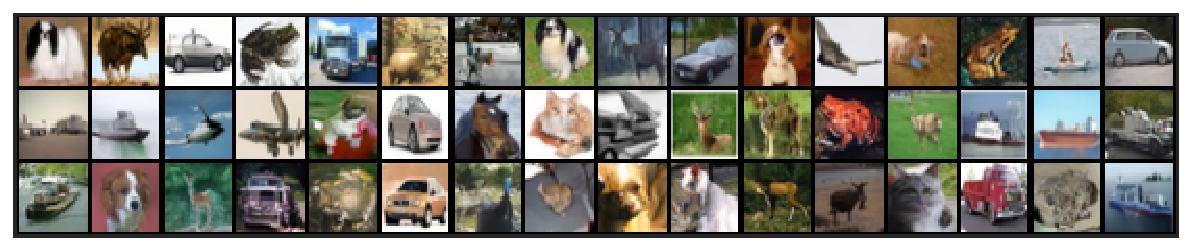
\includegraphics[width=0.8\textwidth]{figures/cifar10-samples-uniform-1000-ddpm.pdf}
    \end{subfigure}
    ~
    \begin{subfigure}{\textwidth}
    \centering
    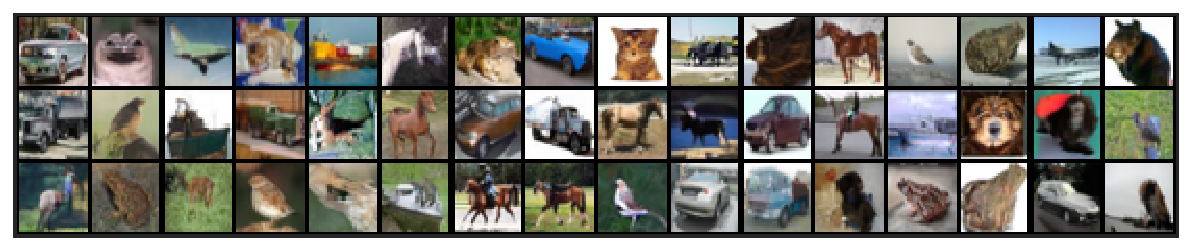
\includegraphics[width=0.8\textwidth]{figures/cifar10-samples-pt-1000-ddim.pdf}
    \end{subfigure}
    ~
    \begin{subfigure}{\textwidth}
    \centering
    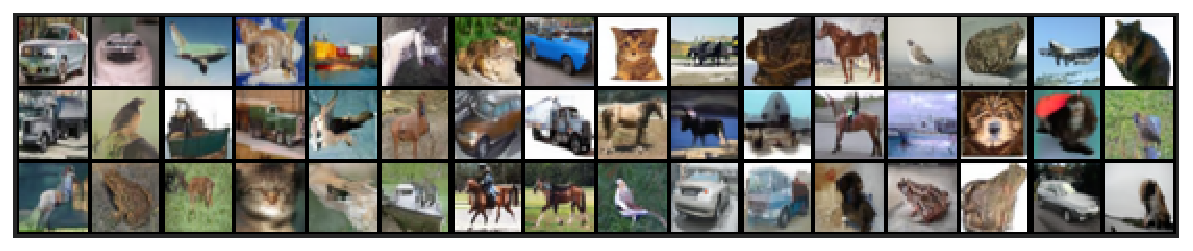
\includegraphics[width=0.8\textwidth]{figures/cifar10-samples-quad-100-ddim.pdf}
    \end{subfigure}
    \caption{CIFAR10 samples from 1000 step DDPM, 1000 step DDIM and 100 step DDIM.}
    \label{fig:cifar10-samples}
\end{figure}

\begin{figure}
    \centering
    \begin{subfigure}{\textwidth}
    \centering
    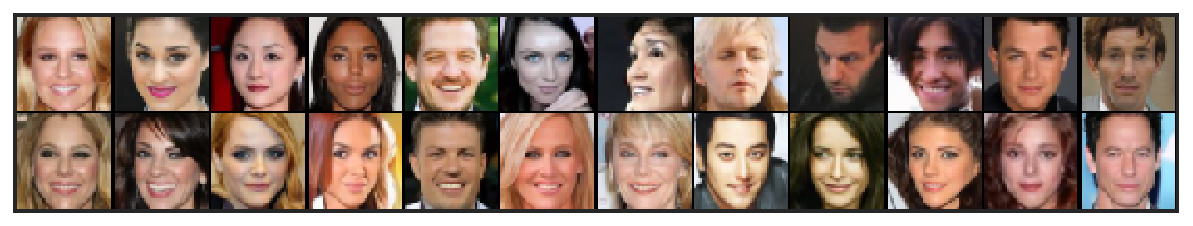
\includegraphics[width=0.8\textwidth]{figures/celeba-samples-uniform-1000-ddpm.pdf}
    \end{subfigure}
    ~
    \begin{subfigure}{\textwidth}
    \centering
    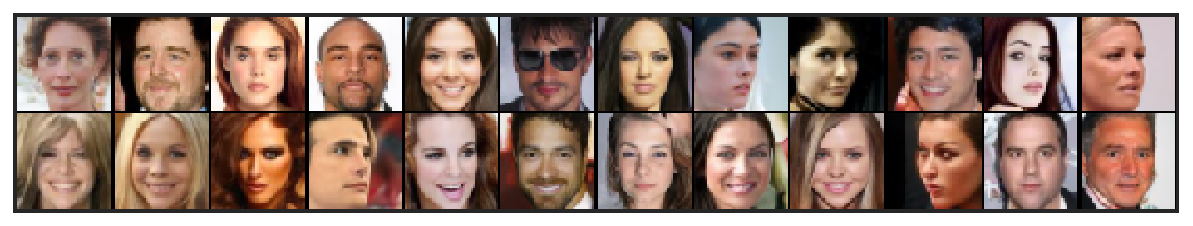
\includegraphics[width=0.8\textwidth]{figures/celeba-samples-uniform-1000-ddim.pdf}
    \end{subfigure}
    ~
    \begin{subfigure}{\textwidth}
    \centering
    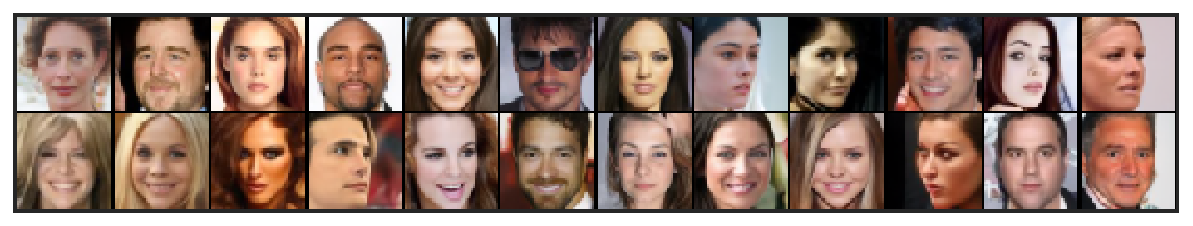
\includegraphics[width=0.8\textwidth]{figures/celeba-samples-uniform-100-ddim.pdf}
    \end{subfigure}
    \caption{CelebA samples from 1000 step DDPM, 1000 step DDIM and 100 step DDIM.}
    \label{fig:celeba-samples}
\end{figure}

\begin{figure}
    \centering
    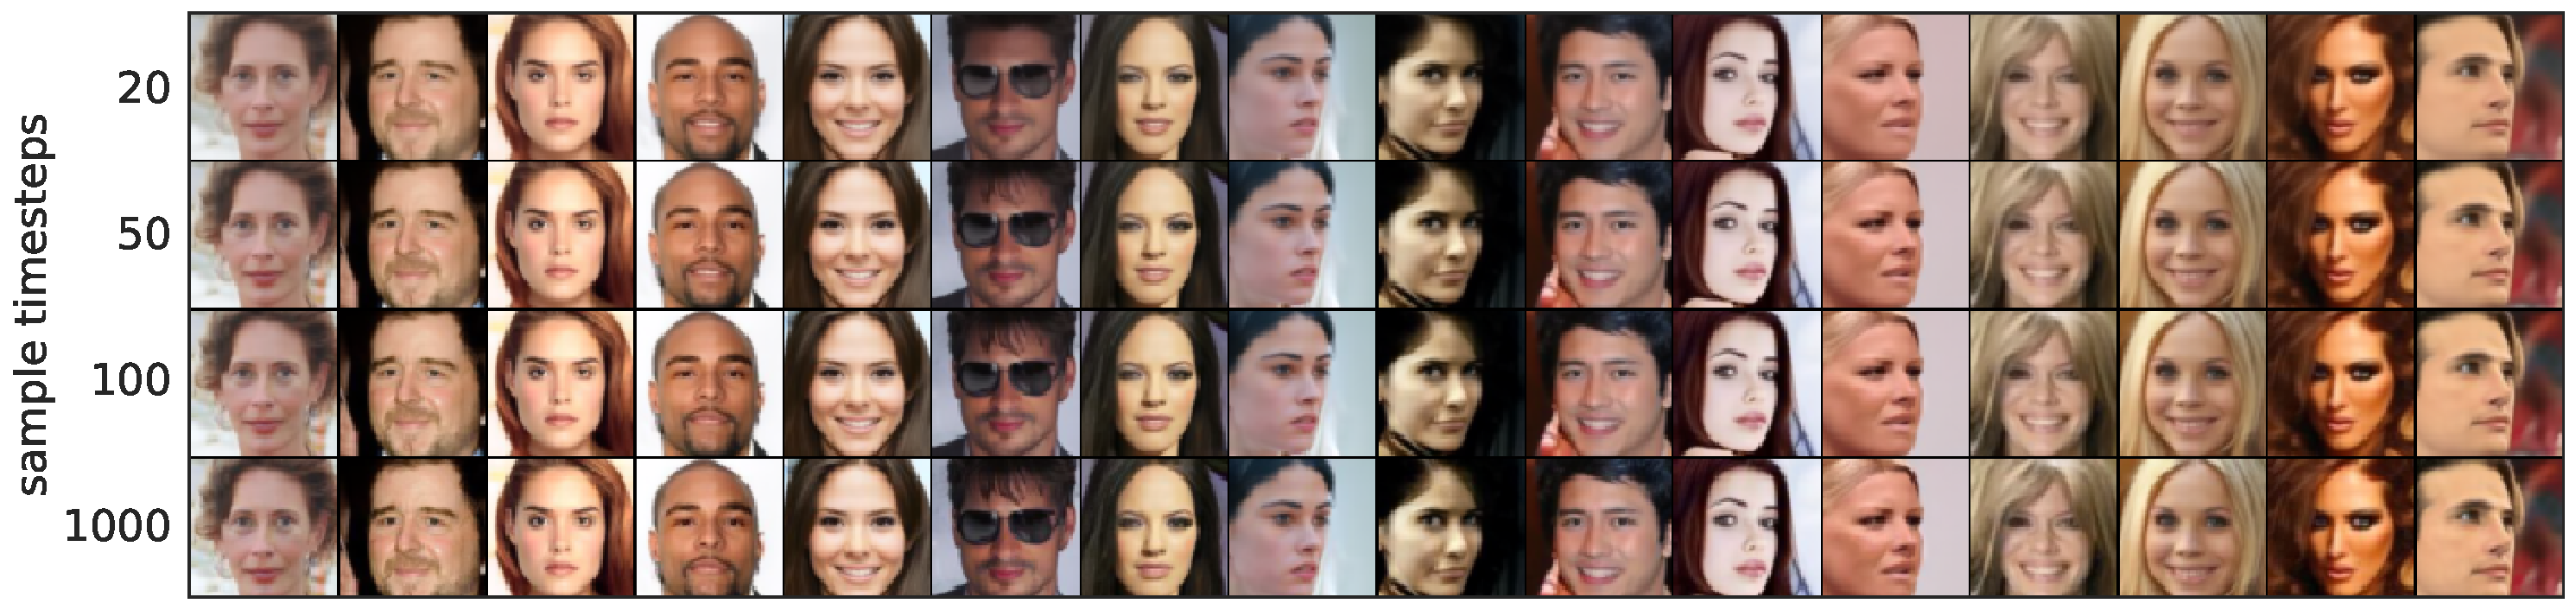
\includegraphics[width=\textwidth]{figures/celeba-consistency.pdf}
    \caption{CelebA samples from DDIM with the same random $\vx_T$ and different number of steps.}
    \label{fig:celeba-consistency}
\end{figure}

\begin{figure}
    \centering
    \begin{subfigure}{\textwidth}
    \centering
    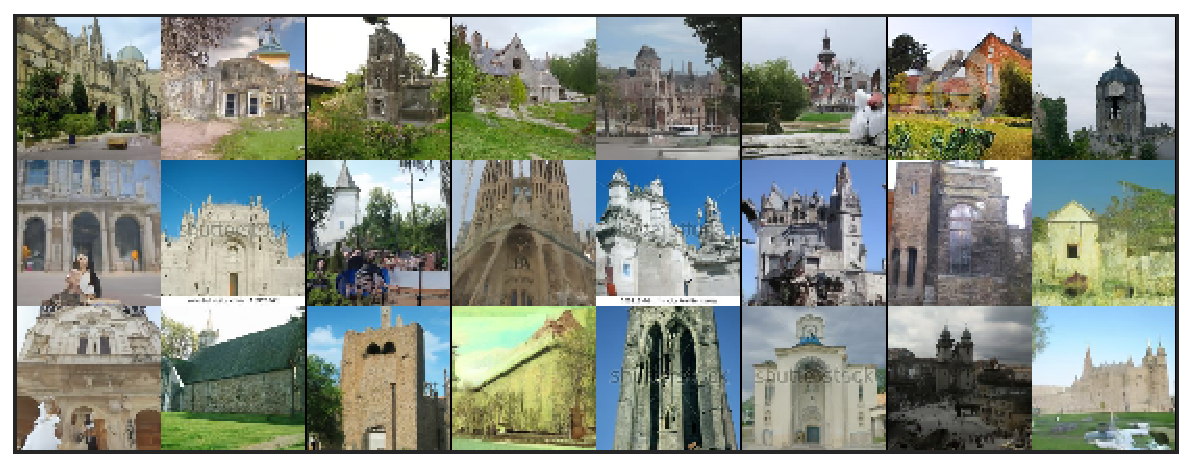
\includegraphics[width=0.8\textwidth]{figures/church-samples-uniform-100-ddpm.pdf}
    \end{subfigure}
    ~
    \begin{subfigure}{\textwidth}
    \centering
    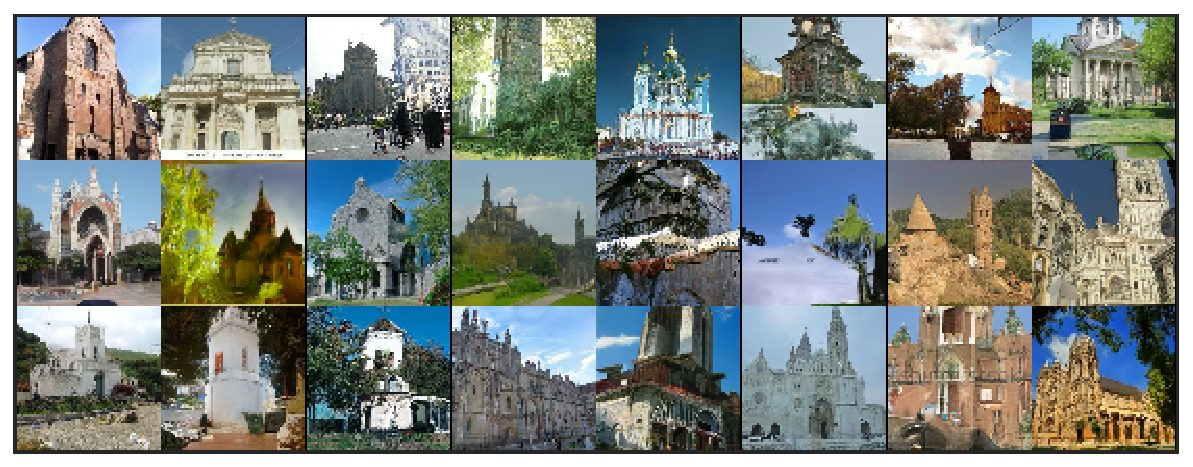
\includegraphics[width=0.8\textwidth]{figures/church-samples-uniform-100-ddim.pdf}
    \end{subfigure}
    \caption{Church samples from 100 step DDPM and 100 step DDIM.}
    \label{fig:church-samples}
\end{figure}



\subsection{Interpolation}
\label{app:interpolation}
To generate interpolations on a line, we randomly sample two initial $\vx_T$ values from the standard Gaussian, interpolate them with spherical linear interpolation \citep{shoemake1985animating}, and then use the DDIM to obtain $\vx_0$ samples.
\begin{align}
    \vx_T^{(\alpha)} =  \frac{\sin((1 - \alpha) \theta)}{\sin(\theta)} \vx_{T}^{(0)} + \frac{\sin(\alpha \theta)}{\sin(\theta)} \vx_{T}^{(1)}
\end{align}
where $\theta = \arccos\left(\frac{(\vx_T^{(0)})^\top \vx_T^{(1)}}{\norm{\vx_T^{(0)}} \norm{\vx_T^{(1)}}}\right)$. These values are used to produce DDIM samples.

To generate interpolations on a grid, we sample four latent variables and separate them in to two pairs; then we use slerp with the pairs under the same $\alpha$, and use slerp over the interpolated samples across the pairs (under an independently chosen interpolation coefficient). We show more grid interpolation results in \Figref{fig:celeba-interp-grid} (CelebA), \Figref{fig:bedroom-interp-grid} (Bedroom), and \Figref{fig:church-interp-grid} (Church).

\begin{figure}[htbp]
    \centering
    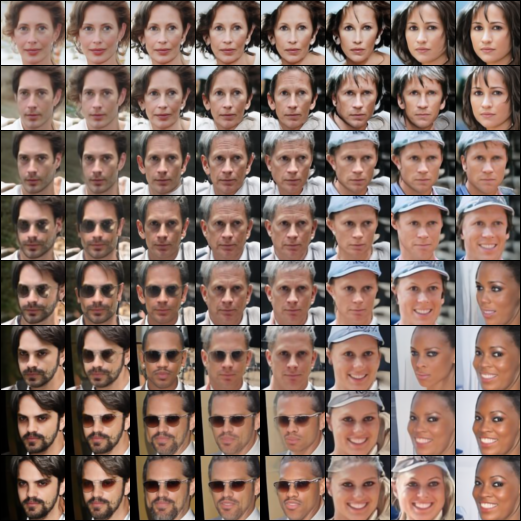
\includegraphics[width=0.6\textwidth]{figures/celeba-interp-grid.png}
    \caption{More interpolations from the CelebA DDIM with $\dim(\tau) = 50$.}
    \label{fig:celeba-interp-grid}
\end{figure}

\begin{figure}[htbp]
    \centering
    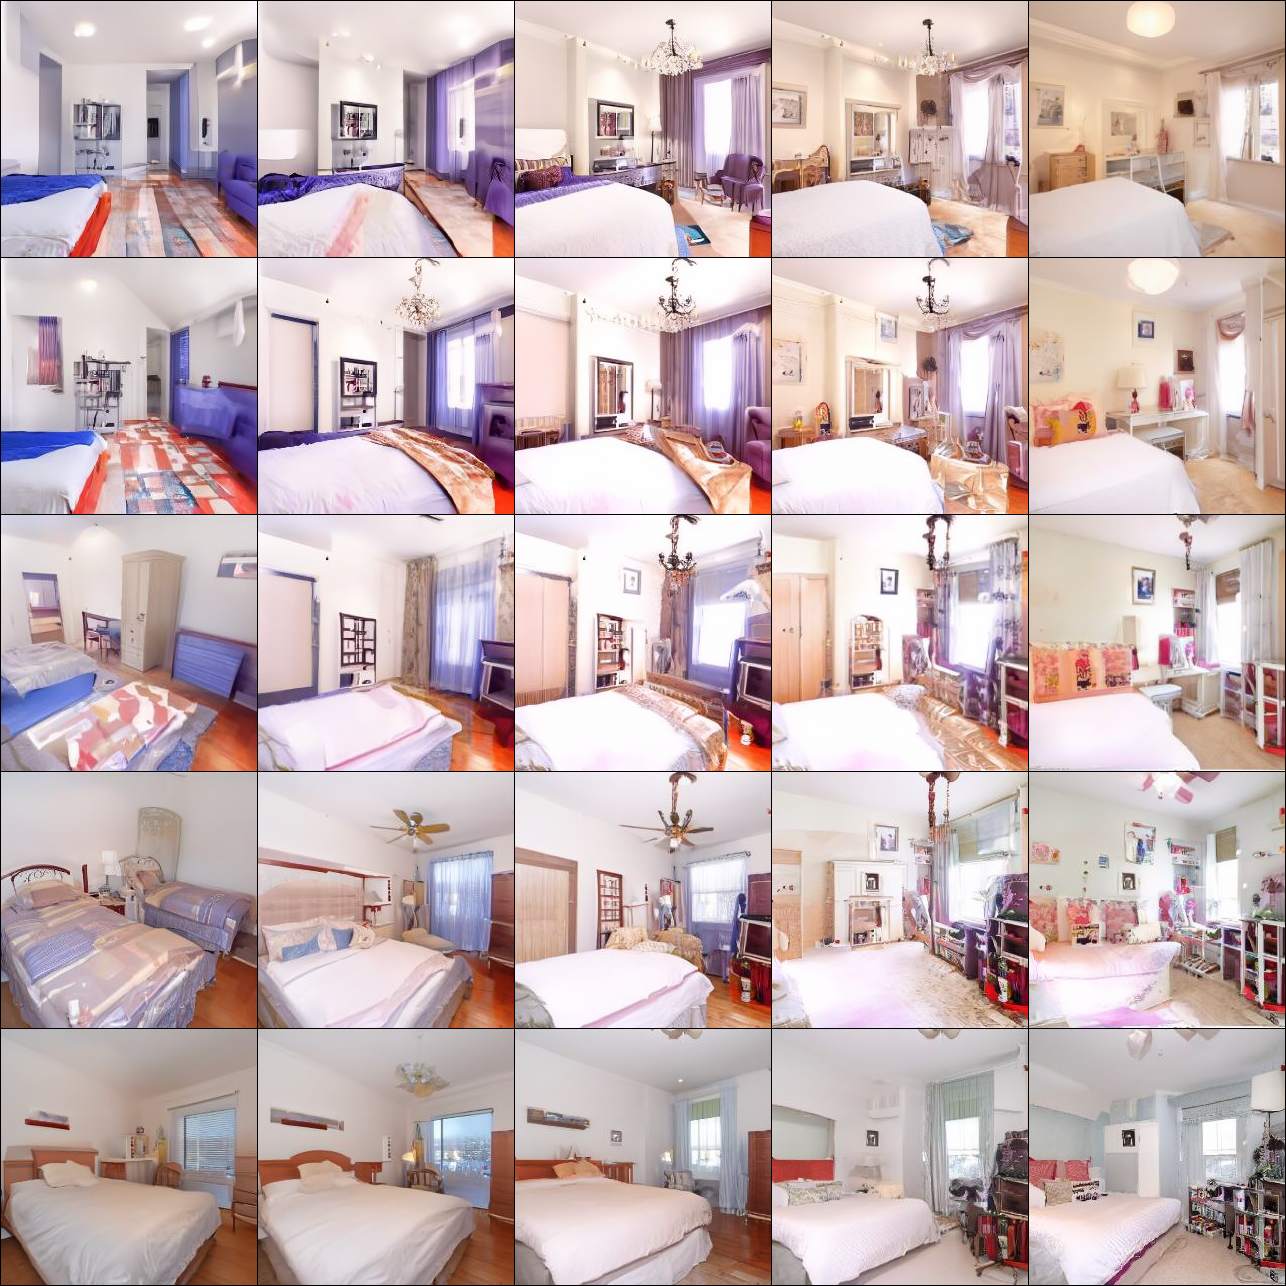
\includegraphics[width=0.6\textwidth]{figures/bedroom-interp-grid.png}
    \caption{More interpolations from the Bedroom DDIM with $\dim(\tau) = 50$.}
    \label{fig:bedroom-interp-grid}
\end{figure}

\begin{figure}[htbp]
    \centering
    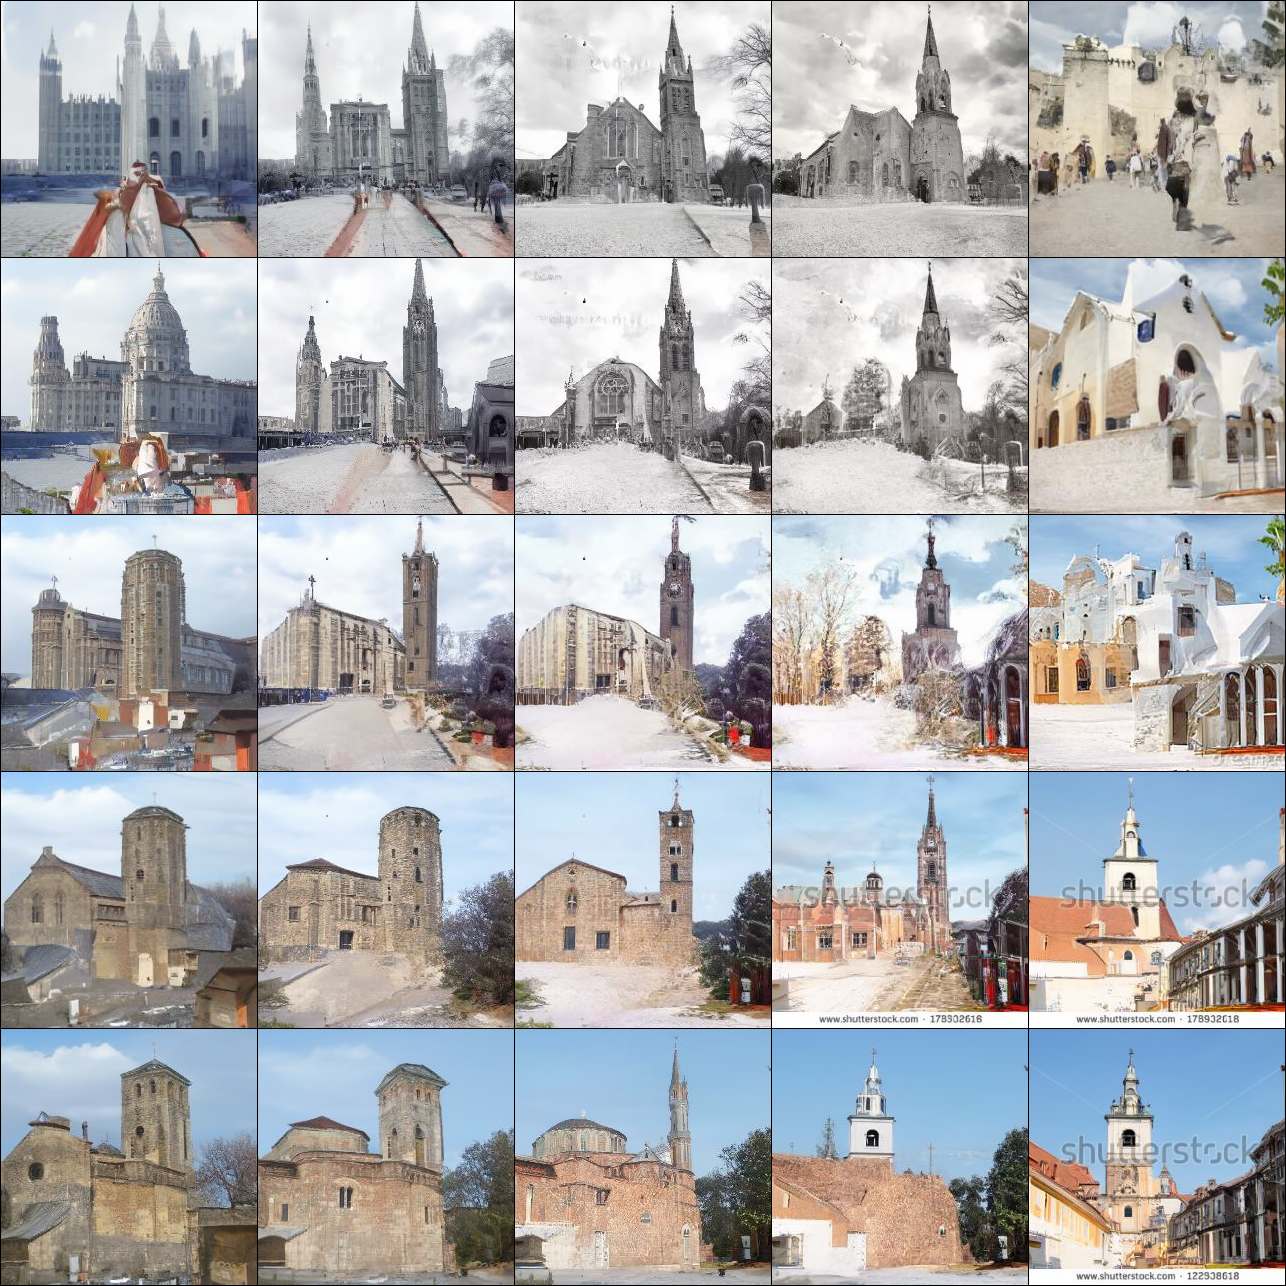
\includegraphics[width=0.6\textwidth]{figures/church-interp-grid.png}
    \caption{More interpolations from the Church DDIM with $\dim(\tau) = 50$.}
    \label{fig:church-interp-grid}
\end{figure}